\documentclass{article}
\usepackage[utf8]{inputenc}
\usepackage[spanish]{babel}
\usepackage{listings}
\usepackage{graphicx}
\graphicspath{ {images/} }
\usepackage{cite}

\begin{document}

\begin{titlepage}
    \begin{center}
        \vspace*{1cm}
            
        \Huge
        \textbf{Calistenia (Parcial 1)}
            
        \vspace{0.5cm}
        \LARGE
        Instrucciones.
            
        \vspace{1.5cm}
            
        \textbf{Juan Fernando Muñoz López}
            
        \vfill
            
        \vspace{0.8cm}
            
        \Large
        Despartamento de Ingeniería Electrónica y Telecomunicaciones\\
        Universidad de Antioquia\\
        Medellín\\
        Marzo 9 de 2021
            
    \end{center}
\end{titlepage}

\tableofcontents
\newpage
\section{El reto de las tarjetas: }\label{intro}
La capacidad de los seres humanos para poder completar sus objetivos, logra ser más grande que su misma capacidad intelectual; pues sin importar el reto, hace lo posible por cumplirlo. En esta ocasión comprobaremos que tan obstinada es tu valía, para llevar a cabo un sencillo pero demandante reto; que consiste en llevar dos tarjetas de cierta posición (A) a otra posición (B) con una sola mano. A continuación, te socializaré los pasos a seguir para que juntos podamos lograrlo.

\section{Instrucciones: } \label{contenido}
Nuestro objetivo principal será llevar dos tarjetas de tamaños similares, las cuales se encuentran debajo de una hoja de papel, con el fin de que ambas estén alineadas encima de la hoja, formando así una figura piramidal.
\subsection{Elementos necesarios}
Para desarrollar nuestro ejercicio necesitaremos de:
\newline 

- Dos \textbf{tarjetas} de tamaño y peso similar.
\newline

- Una \textbf{hoja de papel} completamente lisa.
\begin{figure}[h]
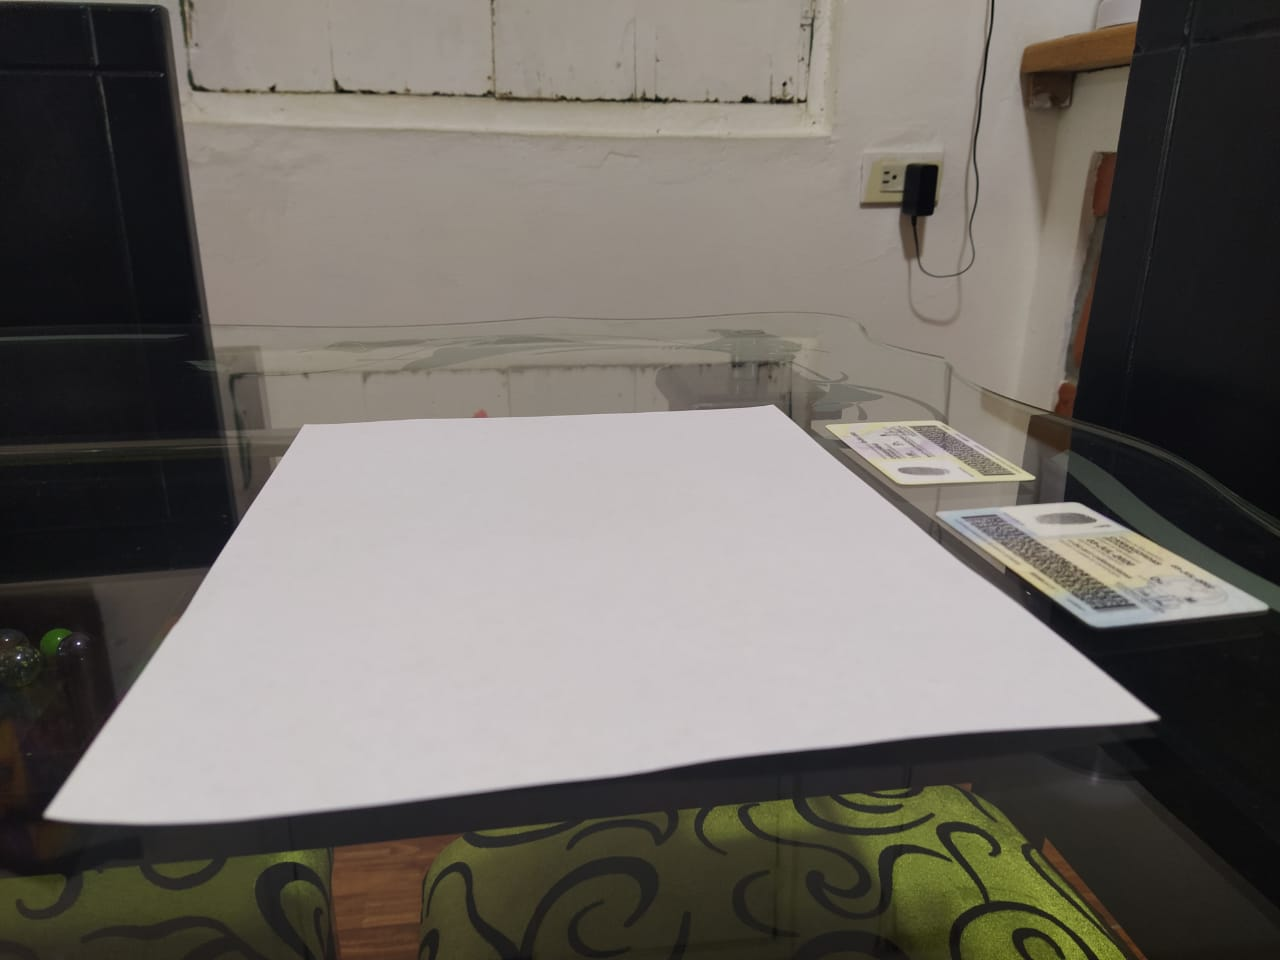
\includegraphics[width=5cm]{elementos.jpeg}
\centering
\caption{Elementos necesarios para la actividad.}
\label{fig:elementos}
\end{figure}
\newline

-Es necesario conocer el nombre de los dedos de la \textbf{mano} para seguir correctamente la instrucción, para ello, en la siguiente imagen se te socializará esta valiosa información \cite{dedosmano}.
\newpage
\begin{figure}[h]
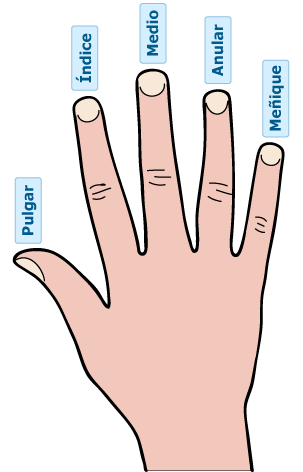
\includegraphics[width=4cm]{nombre_dedos_mano (1).png}
\centering
\caption{Dedos de la mano.}
\label{fig:fingers}
\end{figure}
\subsection{Desarrollo del ejercicio (Tomar las tarjetas): }
Para este ejercicio se necesitará habilidad motriz, puesto que utilizaremos una sola mano, haremos uso de aquella con 
la que nos sintamos más cómodos
.
\newline

\begin{figure}[h]
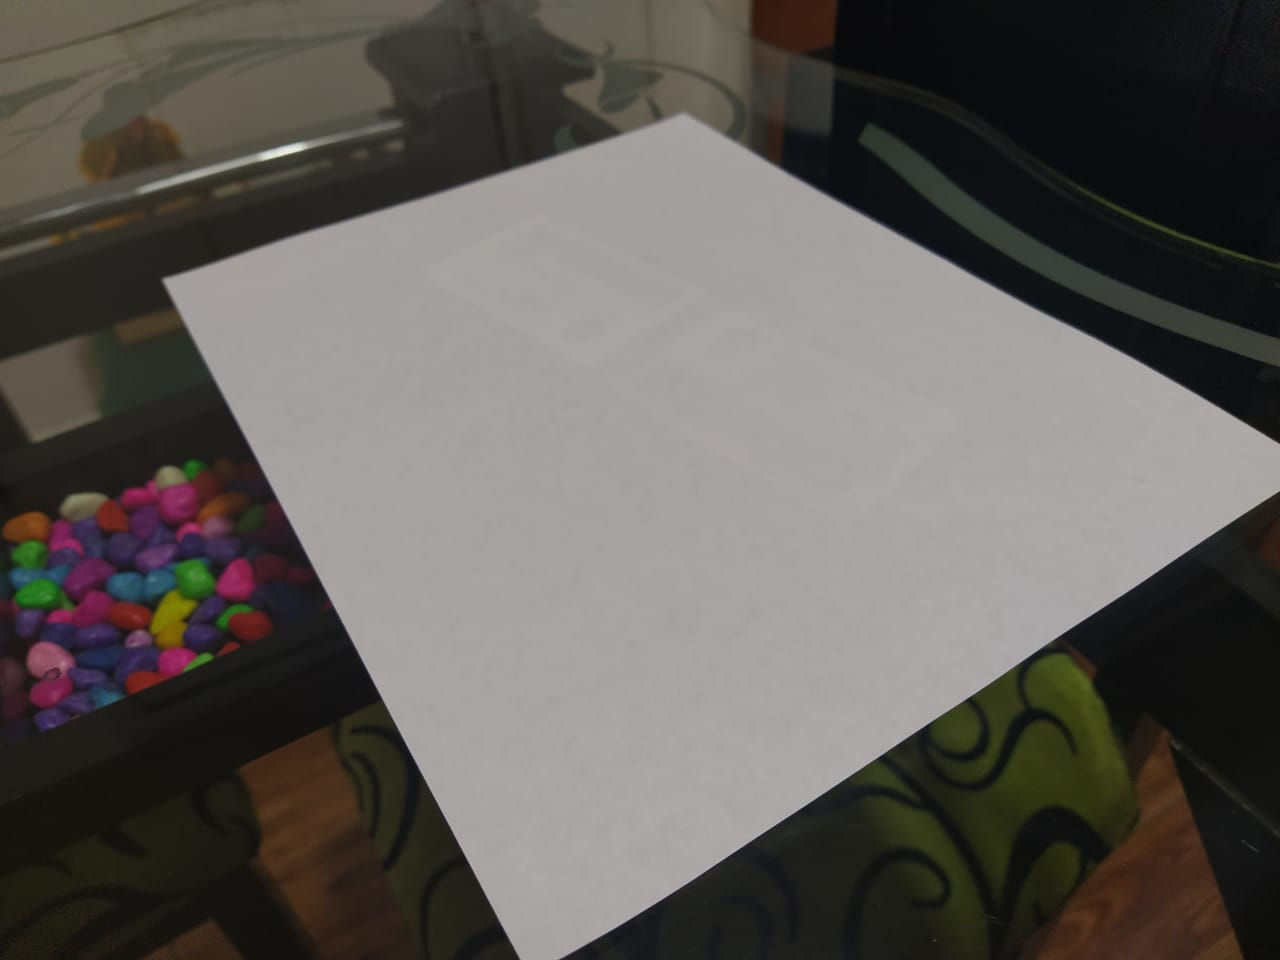
\includegraphics[width=5cm]{estado inicial.jpeg}
\centering
\caption{Estado inicial.}
\label{fig:inicial}
\end{figure}

\textbf{2.2.1 :} Como las tarjetas están debajo de la hoja, lo primero que vamos a hacer es tomar la     hoja    para acceder a las tarjetas, si hay algún tipo de dificultad a la hora de          levantar la            hoja, se puede se seguir la siguiente sugerencia, de lo contario pasar al paso 2.3.
\newline

\textbf{2.2.2 :} Lo primero que debemos hacer es ubicar empleando el uso de los dedos Pulgar y el Índice, el pulgar lo ubicaremos en una esquina de la hoja haciendo algo de presión, posteriormente el dedo índice lo ubicaremos en el lugar más cercano en dirección al centro de la hoja posible, (no es necesario que estos estén demasiado lejos uno del otro). Para finalizar, deslizaremos el dedo pulgar hacia el dedo índice levantando simultáneamente la hoja de papel.


\newline

\subsection{Desarrollo del ejercicio (Alinearlas de forma triangular): } 
\newline

\textbf{2.3.1 :}  Con la ayuda de nuestro mano más hábil, vamos a tomar ambas
tarjetas, para posteriormente ponerlas de manera alineada como si estuviera
percibiendo a una sola, de tal manera que estas se encuentren sobre nuestra
palma, donde uno de los extremos más pequeños debe apuntar hacia tu pulgar, durante este proceso la palma de la mano debe estar boca arriba.
\newline
   
\textbf{2.3.2 :} Teniendo las tarjetas en la palma de la mano las deslizaremos hacia los cuatro dedos superiores. Con nuestro pulgar vamos a deslizar una de las tarjetas en dirección al dedo del medio, para separarla y sostenerla con el pulgar y el dedo medio (dejando la otra sobre la palma); a continuación, la tarjeta que hemos separado con anterioridad, la terminaremos de separar con los dedos meñique y anular. Además, estos el dedo meñique y el anular, separarán las dos tarjetas por dentro, mientras que el dedo el medio, anular y pulgar están por fuera, logrando así una forma piramidal (los extremos superiores pequeños tienen contacto y los extremos inferiores no) las acercaremos a la hoja y las colocaremos de forma vertical.
\newline
   
\textbf{2.3.2 :} Una vez nuestras tarjetas hagan contacto con la hoja de papel, deslizaremos nuestros dedos meñique y anular hacia la parte superior, intentaremos que nuestras tarjetas se encuentren distanciadas, el objetivo es variar la distancia para que estas puedan estar en equilibrio de manera más sencilla, y así lograr una forma piramidal o triangular. Con extremo cuidado intentaremos separar todos nuestros dedos de las tarjetas para que estas se mantenga en equilibrio. De esta manera lograremos consolidar el objetivo principal.
\begin{figure}[h]
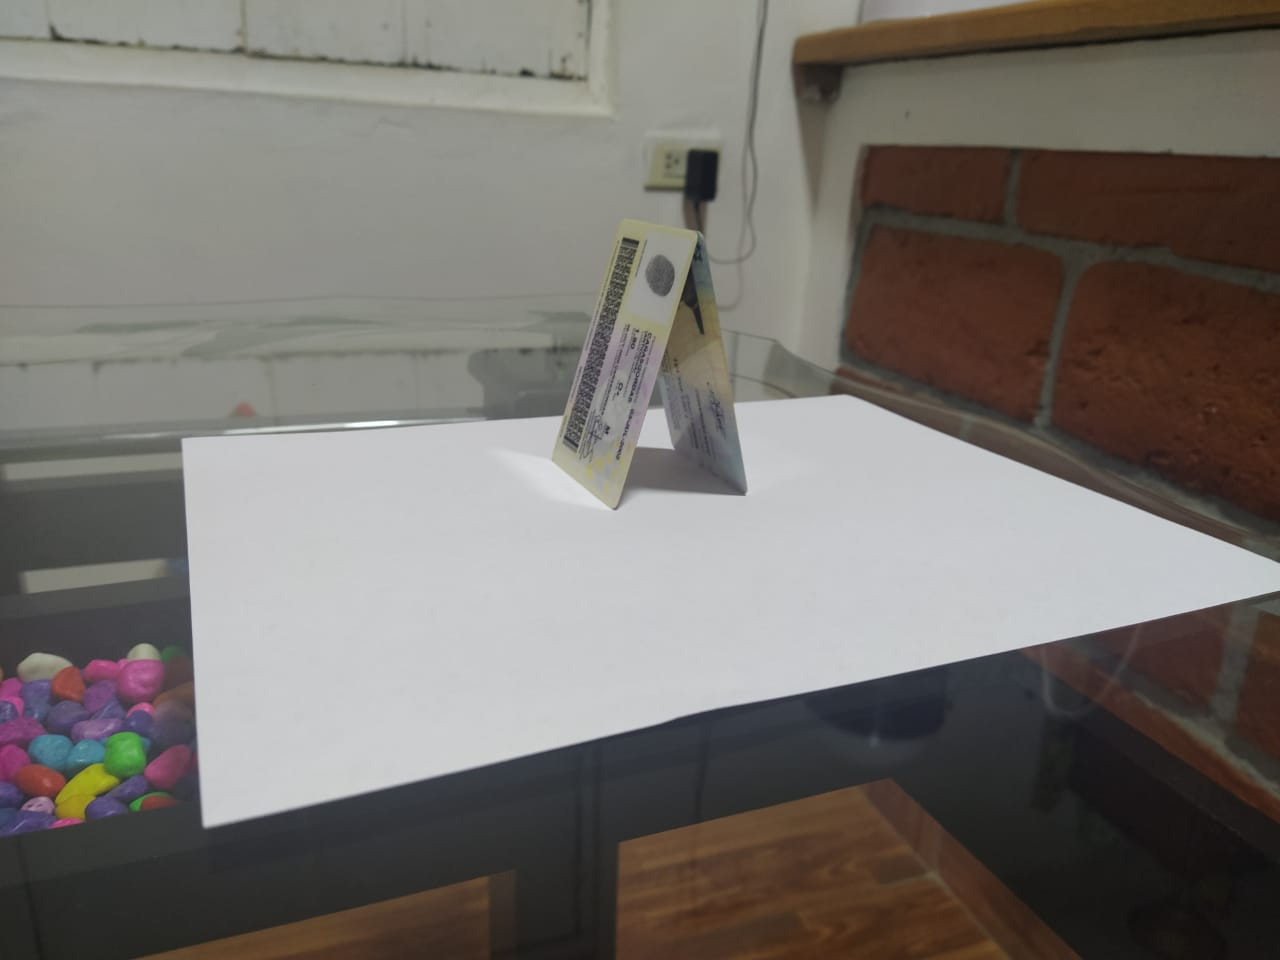
\includegraphics[width=5cm]{WhatsApp Image 2021-03-06 at 3.46.25 PM.jpeg}
\centering
\caption{Estado final.}
\label{fig:final}
\end{figure}

\bibliographystyle{IEEEtran}
\bibliography{references}

\end{document}
